%(BEGIN_QUESTION)
% Copyright 2008, Tony R. Kuphaldt, released under the Creative Commons Attribution License (v 1.0)
% This means you may do almost anything with this work of mine, so long as you give me proper credit

{\it Deriveringskretser} gir en utgangsspenning som er proporsjonal med {\it endringshastigheten over tid} til inngangsspenningen. Det vil si at utgangen fra en deriveringskrets gjenspeiler hvor {\it raskt} inngangsspenningen endrer seg.

$$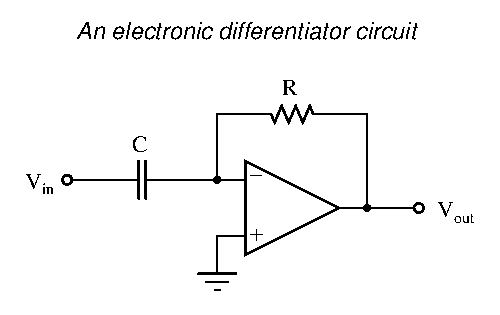
\includegraphics[width=15.5cm]{i01577x01.eps}$$

$$U_{out} = -\tau_d {dU_{in} \over dt}$$

Hver deriveringskrets har en {\it tidskonstant} ($\tau_d$), av og til kalt {\it karakteristisk tid}, som er en proporsjonalitetskonstant mellom inngangens endringshastighet (målt i volt per sekund) og utgangsspenningen (målt i volt). For eksempel vil en deriveringskrets som den vist over, med tidskonstant 3 sekunder, gi en konstant utgangsspenning på -15 volt dersom inngangsspenningen stiger med 5 volt per sekund:

$$-15 \hbox{ [V]} = -\left(3 \hbox{ [s]}\right) \left({5 \hbox{ [V]}\over \hbox{[s]}}\right) $$

\vskip 10pt

{\it Integratorkretser} har også tidskonstanter ($\tau_i$), som uttrykker en proporsjonalitet mellom én spenning og en annen spennings endringshastighet. Forklar hvordan tidskonstanten til en elektronisk integratorkrets kan beregnes fra komponentverdiene, og lag deretter et ``tankeeksperiment'' der du anvender forklaringen din på følgende integratorkrets, slik at du viser hva tidskonstanten betyr i praksis:

$$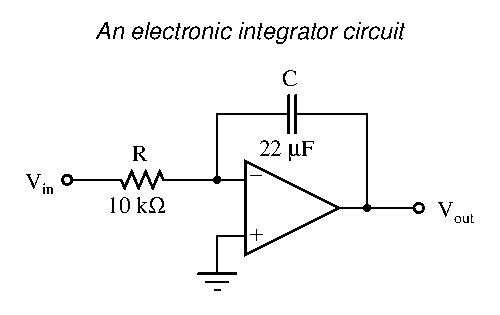
\includegraphics[width=15.5cm]{i01577x02.eps}$$

\vskip 20pt \vbox{\hrule \hbox{\strut \vrule{} {\bf Forslag til sokratisk diskusjon} \vrule} \hrule}

\begin{itemize}
\item{} En nyttig problemløsningsteknikk ved kvalitative eller konseptuelle spørsmål er å sette inn tallverdier i oppgaven, slik at du får noe konkret å regne på. Prøv denne teknikken her.
\item{} Finn flere måter å {\it øke} tidskonstanten for en av kretsene på.
\item{} Av disse måtene, hvilken tror du er enklest å gjennomføre i en praktisk krets? Forklar hvorfor.
\item{} Anta at et konstant DC-spenningssignal på 2 volt legges på inngangen til denne integratorkretsen i 1.5 sekunder. Deretter går inngangssignalet til null og blir der. Hva vil utgangen fra denne opamp-kretsen gjøre, dersom den startet på 0 volt før vi la inn DC-signalet?
\item{} Gitt et konstant DC-spenningssignal på 2 volt inn på denne integratorkretsen, beregn alle strømmer og spenningsfall i kretsen. Marker tydelig alle strømretninger og spenningspolaritetene.
\end{itemize}

\underbar{file i01577}
%(END_QUESTION)





%(BEGIN_ANSWER)

$\tau_i = RC$, akkurat som $\tau_d = RC$ i en deriveringskrets.

$$U_{in} = -\tau_i {dU_{out} \over dt} \hbox{\hskip 40pt eller \hskip 40pt} {dU_{out} \over dt} = -{U_{in} \over \tau_i} \hbox{\hskip 40pt eller \hskip 40pt} U_{out} = -{1 \over {\tau_i}} \int U_{in} \> dt$$

Hva ``tidskonstanten'' betyr i praksis for en integratorkrets, er den tiden det tar for utgangen å stige (eller falle) med like mange volt som inngangen har. En annen måte å si dette på er at tidskonstanten er tiden kretsen bruker på å {\it gjenta} inngangsspenningen.

%(END_ANSWER)





%(BEGIN_NOTES)

Med $R$ = 10 k$\Omega$ og $C$ = 22 $\mu$F blir tidskonstanten for integratorkretsen $\tau = RC$ = 0.22 sekunder. Dette betyr at hvis vi legger inn en konstant DC-spenning på 1 volt, vil utgangsspenningen i denne kretsen endre seg med 1 volt hver 0.22 sekund, som tilsvarer 4.5454 volt per sekund.

Hvis vi legger inn et signal på 2 VDC i inngangen til denne kretsen, vil utgangen rampe lineært med 9.0909 volt per sekund. Dersom denne tilstanden varer i 1.5 sekunder, vil utgangen endres totalt 13.6364 volt fra startverdien. Presist sagt vil utgangen gå {\it ned} 13.6364 volt fra startpunktet på null, fordi dette er en {\it inverterende} opamp-krets.

\vskip 10pt

Press studentene til å lage sitt eget ``tankeeksperiment'' som illustrerer hva ``tidskonstant'' betyr for en integratorkrets. Poenget med øvelsen er å få dem til å begrepsfeste ideen om ``sekunder per {\it gjentakelse}'', slik integralkoeffisienten ofte uttrykkes i PID-regulatorer.









\vfil \eject

\noindent
{\bf Oppsummeringsquiz:}

Bestem hva utgangsspenningen i denne kretsen vil gjøre når inngangen får et konstant DC-spenningssignal:

$$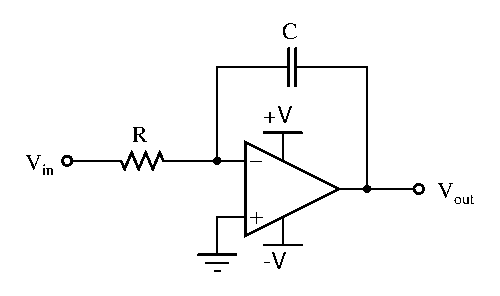
\includegraphics[width=15.5cm]{i01577x03.eps}$$

\begin{itemize}
\item{} Utgangsspenningen vil rampe med konstant hastighet
\vskip 5pt 
\item{} Utgangsspenningen vil minke til den når null volt
\vskip 5pt 
\item{} Utgangsspenningen vil holde seg stabilt på null volt
\vskip 5pt 
\item{} Utgangsspenningen vil rampe med økende hastighet (som en krummet skihoppbakke)
\vskip 5pt 
\item{} Utgangsspenningen vil holde seg stabil på en verdi lik inngangen
\vskip 5pt 
\item{} Utgangsspenningen vil oscillere fram og tilbake (AC)
\end{itemize}


%INDEX% Electronics review: differentiator versus integrator circuits

%(END_NOTES)
